% !TeX program = lualatex

\documentclass[a4paper,12pt]{article}
%Monday May 30, 2022 at 17:00 CEST
\PassOptionsToPackage{hyphens}{url}
\usepackage[
  backend=biber,
  defernumbers=true,
  sorting=none,
  style=numeric-comp,
  natbib=true,
  url=false,
  giveninits=true,
  hyperref,
  eprint=true,
  doi=true
]{biblatex}
\renewbibmacro{in:}{}
\usepackage{makecell}
\usepackage{lastpage}
\usepackage{csquotes}
\addbibresource{refs.bib}
\usepackage[top=4.5cm, bottom=2.9cm, left=2.1cm, right=2.1cm]{geometry}
\usepackage{xltabular}
\usepackage{tabulary}
\usepackage{enumitem}
\usepackage{hyperref}
\hypersetup{colorlinks=true,allcolors=blue}
\usepackage{pgfgantt}
\usepackage{hypcap}
\usepackage{fancyhdr}
\usepackage{graphicx}
\usepackage{xcolor}
\usepackage{colortbl}
\usepackage[english]{babel}
\usepackage{lastpage}
\usepackage{slashed}
\usepackage{fontspec}
\usepackage{unicode-math}
\usepackage{dblfnote} % multicolumn footnotes
\defaultfontfeatures{ Scale=MatchLowercase, Ligatures = TeX }
\setmainfont{Arial}
\setsansfont{Arial}
\setmonofont{Courier New Bold}[Scale=0.9]
\usepackage{wasysym}
\usepackage{lipsum}
\usepackage[linecolor=blue]{mdframed}
% needed for definite figure placement using [H]
\usepackage{float}
\usepackage{sidecap}

\usepackage{cleveref}

\pagestyle{fancy}
\usepackage{ifthen}
\usepackage{titlesec}
\usepackage{wrapfig}
\usepackage{multirow}
\usepackage{caption}
\usepackage{textcomp}
\captionsetup{font=small}

\usepackage{xfp}
\usepackage{calc}

\newlength\myheight
\newlength\mydepth
\settototalheight\myheight{Xygp}
\settodepth\mydepth{Xygp}
\setlength\fboxsep{0pt}
\newcommand*\inlinegraphics[1]{%
  \settototalheight\myheight{Xygp}%
  \settodepth\mydepth{Xygp}%
  \raisebox{-\mydepth}{\includegraphics[height=\myheight]{#1}}%
}

\let\oldbibliography\thebibliography
\renewcommand{\thebibliography}[1]{%
  \oldbibliography{#1}%
  \setlength{\itemsep}{0pt}%
}

\setcounter{secnumdepth}{4}
\newcommand{\MSb}{\overline{\mathrm{MS}}}
\newcommand{\Dsla}{\slashed{D}}
\newcommand{\Dlr}{\buildrel \leftrightarrow \over D\raise-1pt\hbox{}}
\DeclareFieldInputHandler{title}{\def\NewValue{}}
\setlength\bibitemsep{1.5\itemsep}

\newif\ifshowinstructions
\newcommand{\instructions}[1]{\ifshowinstructions {\fontsize{10}{11}\selectfont \textit{#1}} \fi}

\newcommand{\RF}[1]{\textbf{\color{magenta}RF: #1}}
\newcommand{\SB}[1]{\textbf{\color{red}SB: #1}}

\usepackage[user]{zref}

\newcounter{pageaux}
\def\currentauxref{PAGEAUX1}
\makeatletter
\newcommand{\resetpageaux}{%
  \clearpage
 \edef\@currentlabel{\thepageaux}\label{\currentauxref}%
  \xdef\currentauxref{PAGEAUX\thepage}%
  \setcounter{pageaux}{0}}
\AtEndDvi{\edef\@currentlabel{\thepageaux}\label{\currentauxref}}
\makeatother

%% this is a hack required by xelatex, which seems to always render the text inside
%% an mdframed in black... 
\newenvironment{jubox}
  {
    \begin{mdframed}
    \globalcolor{blue}
  }
  {
    \end{mdframed}
  }


\titleformat{\section}
  {\normalfont\fontsize{14}{16.8}\bfseries\selectfont}{\thesection}{1em}{}[{\color{oliv}\titlerule[1pt]}]

\titleformat{\subsection}
  {\normalfont\fontsize{14}{16.8}\selectfont}{\thesubsection}{1em}{}[{\color{oliv}\titlerule[1pt]}]

\titleformat{\subsubsection}
  {\normalfont\it\fontsize{14}{16.8}\selectfont}{\thesubsubsection}{0.8em}{}[{\color{orng}\titlerule}]

\titleformat{\paragraph}%[runin]
  {\normalfont\fontsize{14}{16.8}\selectfont}{\theparagraph}{0.5em}{}%[: \qquad]

\titlespacing*{\section}{0pt}{0pt}{0pt}
\titlespacing*{\subsection}{0pt}{0pt}{6pt}
\titlespacing*{\subsubsection}{0pt}{0pt}{0pt}
\titlespacing*{\paragraph}{0pt}{0pt}{0pt}

\definecolor{blue}{HTML}{19317B}
\definecolor{orng}{HTML}{FFC000}
\definecolor{oliv}{HTML}{FFC000}
\definecolor{lblu}{HTML}{4F81BD}
\definecolor{llbl}{HTML}{DBE5F1}

\definecolor{darkred}{HTML}{9f1313}
\definecolor{alizarin}{rgb}{0.82, 0.1, 0.26} % red
\definecolor{bluegray}{rgb}{0.4, 0.6, 0.8} % blue
\definecolor{bittersweet}{rgb}{1.0, 0.44, 0.37}
\definecolor{forestgreen(web)}{rgb}{0.13, 0.55, 0.13}


\setlength{\belowcaptionskip}{6pt}
\setlength{\voffset}{-1in}
\setlength{\topmargin}{0pt}
\setlength{\headheight}{1.2in}
\setlength{\headsep}{0.5in}
\setlength{\footskip}{0.3in}

\newlength\mylen
\addtolength\mylen{\marginparsep}
\addtolength\mylen{\marginparwidth}
\addtolength\mylen{\hoffset}
\addtolength\mylen{1in}
\fancyheadoffset{\the\mylen}

\fancyhead[L]{}
\fancyhead[R]{}

\fancyhead[C]{
  
\includegraphics[width=1\paperwidth]{head.png}
}
\fancyfoot[L]{\footnotesize\color{blue}
  \stepcounter{pageaux} Page \thepageaux\ of \ref{\currentauxref}
}
\fancyfoot[C]{\footnotesize\color{blue}\textbf{EuroHPC JU} | Development Acccess -- Final Report}
\fancyfoot[R]{\footnotesize\color{blue} 04/04/2023}

\renewcommand{\headrulewidth}{0pt}
\renewcommand{\footrule}{\hbox to\headwidth{\color{orng}\leaders\hrule height \footrulewidth\hfill\par}}
\renewcommand{\footrulewidth}{1pt}

\DeclareBibliographyCategory{fullcited}
\newcommand{\mybibexclude}[1]{\addtocategory{fullcited}{#1}}

\usepackage{xparse}
\NewDocumentCommand\Nf{mgg}{N\textsubscript{f}=#1\IfNoValueTF{#2}{}{+#2}\IfNoValueTF{#3}{}{+#3}}
\NewDocumentCommand\vol{mg}{#1\textsuperscript{3}\IfNoValueTF{#2}{}{×#2}}
\setlength{\parindent}{0cm}

\newcommand{\NP}{{\rm NP}}

%%% Variables related to resource estimate
\newcommand{\hrsBS}{0.8}
\newcommand{\hrsB}{0.6}
\newcommand{\hrsBL}{0.8}
\newcommand{\hrsC}{0.6}
\newcommand{\hrsCL}{0.7}
\newcommand{\hrsD}{0.8}
\newcommand{\hrsDL}{0.6}
\newcommand{\hrsE}{0.7}
\newcommand{\rABS}{0}
\newcommand{\rAB}{120*8*10}
\newcommand{\rABL}{200*32*12}
\newcommand{\rAC}{400*20*13}
\newcommand{\rACL}{410*56*5}
\newcommand{\rAD}{300*32*10}
\newcommand{\rADL}{500*128*3}
\newcommand{\rAE}{700*56*6}
\newcommand{\rBBS}{800*2*20}
\newcommand{\rBB}{800*8*20}
\newcommand{\rBC}{800*20*20}
\newcommand{\rBD}{800*32*20}

% the tables in the report template have very wide vertical spacing
\def\arraystretch{1.5}

\linespread{1}
\setlength{\parskip}{6pt}

% checkbox to select a system in the system list
\newcommand{\checkbox}[1]{%
  \ifthenelse{\equal{#1}{yes}}{$\boxtimes$}{$\Box$}%
}

\makeatletter
\newcommand{\globalcolor}[1]{%
  \color{#1}\global\let\default@color\current@color
}
\makeatother

\AtBeginDocument{\globalcolor{blue}}

%\showinstructionsfalse %% Suppresses template instructions
\showinstructionstrue %% Shows template instructions

\begin{document}

{\fontsize{20}{32} \selectfont\textbf{EuroHPC Joint Undertaking (JU) Development Access}}
{\color{orng}\hrule height 1pt}
{\fontsize{20}{32} \selectfont\textbf{Final Report}}

\section{General Information}

Type of project granted: Development Access -- code development and optimization

\subsection{Proposal ID}

\instructions{Please fill in the information in the box below.}

\begin{jubox}
  %% jubox with xelatex seems to be buggy: need to set the text colour again
  EHPC-DEV-2022D08-013
\end{jubox}

\subsection{Period of access to the EuroHPC JU facilities}

\instructions{Please fill in the information in the box below.}

\begin{tabulary}{\textwidth}{|p{0.47\textwidth}|p{0.47\textwidth}|}
  \hline
  Start date of the allocation (DD/MM/YYYY) & DD/MM/YYYY \\
  \hline
  End date of the allocation (DD/MM/YYYY) & DD/MM/YYYY \\
  \hline
  Duration of extension in months (if applicable) & M \\
  \hline
\end{tabulary}

\subsection{EuroHPC JU system assigned}

\instructions{Plese click once in the box to select it, click again to unselect.}

%% use \checkbox{yes} to draw a checked checkbox
%% use \checkbox{no} to draw an empty checkbox

\begin{tabulary}{\textwidth}{p{0.04\textwidth}p{0.40\textwidth}p{0.04\textwidth}p{0.40\textwidth}}
  \checkbox{no} & Vega CPU (IZUM)               & \checkbox{no} & Vega GPU (IZUM) \\
  \checkbox{no} & Meluxina CPU (LuxProvide)     & \checkbox{no} & Meluxina GPU (LuxProvide) \\
  \checkbox{no} & Karolina CPU (IT4Innovations) & \checkbox{no} & Karolina GPU (IT4Innovations) \\
  \checkbox{no} & Discoverer (Sofia Tech Park)  & \checkbox{no} & Deucalion (MACC) \\
  \checkbox{no} & LUMI-C (CSC)                  & \checkbox{no} & LUMI-G (CSC) \\
  \checkbox{no} & Leonardo Booster (CINECA)     & \checkbox{no} & Leonardo DCGP (CINECA) \\
  \checkbox{no} & Marenostrum5 GPP (BSC)        & \checkbox{no} & MareNostrum5 ACC (BSC)
\end{tabulary}

\subsection{Principal Investigator}

\instructions{Please fill in the information in the table below.}

\begin{tabulary}{\textwidth}{|p{0.23\textwidth}|p{0.7\textwidth}|}
  \hline
  Title & \\
  \hline
  First (Given) Name & \\
  \hline
  Last (Family) Name & \\
  \hline
  E-mail Address & \\
  \hline
\end{tabulary}

\section{Project Information}

\subsection{Project title}

\instructions{Please fill in the information in the box below.}

\begin{jubox}
  Project title
\end{jubox}

\subsection{Main research field(s)}

\begin{tabulary}{\textwidth}{p{0.04\textwidth}p{0.40\textwidth}p{0.04\textwidth}p{0.40\textwidth}}
  \checkbox{no} & Biochemistry, Bioinformatics and Life sciences (LS1, LS2, LS8, LS9) & 
    \checkbox{no} & Fundamental Constituens of Matter (PE2) \\
  \checkbox{no} & Chemical Sciences and Materials (PE3, PE4, PE5) &
    \checkbox{no} & Linguistics, Cognition and Culture (SH3, SH4, SH5, SH6) \\
  \checkbox{no} & Earth System Sciences (PE10) & 
    \checkbox{no} & Mathematics and Computer Sciences (PE1, PE6) \\
  \checkbox{no} & Economics, Finance and management (SH1, SH2)  & 
    \checkbox{no} & Physiology and Medicine (LS3, LS4, LS5, LS6, LS7) \\
  \checkbox{no} & Engineering (PE7, PE8) & 
    \checkbox{no} & Universe Science (PE9)
\end{tabulary}

\subsection{Team members and institutions}

\instructions{Please list all team members and corresponding affiliations that were involved in the project.}

\begin{jubox}
  Person X, Institution Y \\
  Person Z, Institution W
\end{jubox}

\subsection{Summary of the project}

\instructions{Please fill in the field with the same text used in the application form (maximum 300 words).}

\begin{jubox}
  \lipsum[1-3]
\end{jubox}

\section{Main features of the code}

\subsection{Name of the code(s)}

\instructions{Please fill in the information in the box below.}

\begin{jubox}
  Name of the code
\end{jubox}

\subsection{Type of the code distribution}

\instructions{Please fill in the information in the box below (e.g. open source, commercial, academic, etc.).}

\begin{jubox}
\end{jubox}

\subsection{Computational problem executed}

\instructions{Please fill in the information in the box below (e.g. N-body problem, Navier-stoles equation, etc.)}

\begin{jubox}
\end{jubox}

\subsection{Computational method}

\instructions{Please fill in the information in the box below (e.g., FEM, FVM, PIC, spectral methods, etc.)}

\begin{jubox}
\end{jubox}

\subsection{Kind of parallelism used}

\instructions{Please fill in the information in the box below (e.g., MPI, OpenMP, MPI/OpenMP, pthreads, embarassingly parallelism, etc.)}

\begin{jubox}
\end{jubox}

\subsection{Main libraries used, version and lagnuage. Usage of /usr/local libraries.}

\instructions{Please fill in the information in the box below: main libraries (e.g., FFTW, MKL, BLAS, LAPACK, etc.), language (e.g., Fortran, C, C++, etc.).}

\begin{jubox}
\end{jubox}

\subsection{Other software used on the EuroHPC JU systems. Usage of post-processing or pre-processing tools.}

\instructions{Please fill in the information in the box below.}

\begin{jubox}
\end{jubox}

\section{Compilation step}

\subsection{How is the program compiled?}

\instructions{Please fill in the information in the box below (e.g., makefile, script, etc.).}

\begin{jubox}
\end{jubox}

\subsection{Difficulties met to compile, if any, and how they were tackled}

\instructions{Please fill in the information in the box below.}

\begin{jubox}
\end{jubox}

\subsection{Which version of the compiler and version of the MPI library was used?}

\instructions{Please fill in the information in the box below.}

\begin{jubox}
\end{jubox}

\subsection{Were any tools for studying the behaviour of the code used?}

\instructions{Please fill in the information in the box below (e.g., debugger, profiler, etc.).}

\begin{jubox}
\end{jubox}

\section{Execution step}
 
\subsection{How is the program launched?}

\instructions{Please fill in the information in the box below.}

\begin{jubox}
\end{jubox}

\subsection{Difficulties met to launch the code, if any, and how they were tackled}

\instructions{Please fill in the information in the box below.}

\begin{jubox}
\end{jubox}

\section{Communication patterns}

\instructions{If you know which are the main communication patterns used in your code configuration, please select the ones from the mentioned below (click once inthe box to select it, click again to unselect):}

\begin{tabulary}{0.6\textwidth}{p{0.04\textwidth}p{0.54\textwidth}}
  \checkbox{no} & Many point-to-point communications \\
  \checkbox{no} & Many collective communications \\
  \checkbox{no} & Barrier \\
  \checkbox{no} & Reduction \\
  \checkbox{no} & Broadcast \\
  \checkbox{no} & Scatter/gather \\
  \checkbox{no} & All to all
\end{tabulary}

\section{Scalability testing}

\subsection{Summary of the obtained results from the scalability testing}

\instructions{Please show the scaling behaviour of the application. Which progress was achieved? Does it fulfill the set expectations? If not, what were the reasons? (maximum 500 words)}

\begin{jubox}
\end{jubox}

\subsection{Images or graphics showing results from the scalability testing}

\instructions{All tables and figures (including photographs, schemas, graphs and diagrams) should be numbered with Arabic numerals (1, 2,\ldots n) and include a descriptive caption. Please attach the images to this form (minimum resolution 300 dpi).}

\begin{figure}[H]
  \begin{minipage}{0.45\textwidth}
    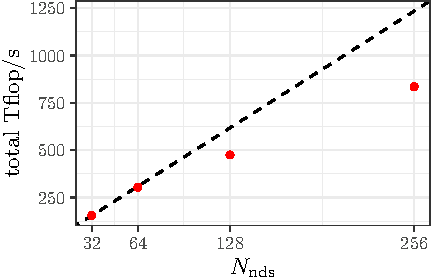
\includegraphics[width=\textwidth,page=1]{scaling1}
  \end{minipage}
  \hfill
  \begin{minipage}{0.45\textwidth}
    \begin{tabulary}{0.45\textwidth}{llll}
      $N_\mathrm{nds}$ & Tflop/s & speedup & efficiency \\
      \hline
      32               & 154.3   & 1.00    & 1.00       \\
      64               & 302.9   & 1.96    & 0.98       \\
      128              & 474.5   & 3.07    & 0.77       \\
      256              & 834.7   & 5.41    & 0.68
    \end{tabulary}
  \end{minipage}
  \caption{\textit{\textbf{Left:} Scaling study of X as a function of the number of nodes. The dashed lined indicates ideal scaling. \textbf{Right:} tabulated data}}
  \label{fig:scaling1}
\end{figure}

\begin{figure}[H]
  \begin{minipage}{0.45\textwidth}
    \includegraphics[width=\textwidth,page=2]{scaling1}
  \end{minipage}
  \hfill
  \begin{minipage}{0.45\textwidth}
    \begin{tabulary}{0.45\textwidth}{llll}
      $N_\mathrm{nds}$ &  Tflop/s & speedup & efficiency \\
      \hline
      32               &  442.6   & 1.00    & 1.00       \\
      64               &  783.3   & 1.77    & 0.88       \\
      128              & 1314.0   & 2.97    & 0.74       \\
      256              & 1751.5   & 3.96    & 0.49
    \end{tabulary}
  \end{minipage}
  \caption{\textit{\textbf{Left:} Scaling study of Y as a function of the number of nodes. The dashed lined indicates ideal scaling. \textbf{Right:} tabulated data}}
  \label{fig:scaling1}
\end{figure}

\subsection{Data to deploy the scalability curves}

\paragraph*{\textbf{A. Typical user test cases}}

\instructions{Please include the data for each test case.}

\begin{tabulary}{0.90\textwidth}{|c|c|c|c|c|}
  \hline
  Number of cores & Wall clock time & Speed-up vs the first one & Number of nodes & Number of processes \\
  \hline
                  &                 &                            &                 &                     \\
  \hline
\end{tabulary}

\paragraph*{\textbf{B. Strong scaling curve}}

\instructions{Please include the data in order to deploy the scalability curve when the number of processors varies for a fixed total problem size.}

\begin{tabulary}{0.90\textwidth}{|c|c|c|c|c|}
  \hline
  Number of cores & Wall clock time & Speed-up vs the first one & Number of nodes & Number of processes \\
  \hline
                  &                 &                            &                 &                     \\
  \hline
\end{tabulary}

\paragraph*{\textbf{C. Weak scaling curve}}

\instructions{Please include the data in order to deploy the scalability curve when the number of processors varies for a fixed problem size per processor.}

\begin{tabulary}{0.90\textwidth}{|c|c|c|c|c|}
  \hline
  Number of cores & Wall clock time & Speed-up vs the first one & Number of nodes & Number of processes \\
  \hline
                  &                 &                            &                 &                     \\
  \hline
\end{tabulary}

\subsection{Publications or reports regarding the scalability testing}

\instructions{Please use the following format: Author(s). ``Title''. Publication, volume, issue, page, month year.}

\begin{jubox}
\end{jubox}

\section{Development and optimization}

\subsection{Summary of the obtained results from the enabling process}

\instructions{Please describe the spent effort. Which progress was achieved? Please describe in detail which enabling work was performed (porting, work on algorithms, I/O…etc.). List problems encountered, if any (maximum 500 words).}

\begin{jubox}
\end{jubox}

\subsection{Used tools for the code analysis, if applicable}

\instructions{Please fill in the information in the box below (e.g., Scalasca, Vampir, etc.) (maximum 500 words).}

\begin{jubox}
\end{jubox}
 
\subsection{Main actions taken for optimization or improvement of codes on the EuroHPC JU systems. Which features were optimized? What were the bottlenecks? Which were the solutions (if any)?}

\instructions{Please fill in the information in the box below (maximum 500 words).}

\begin{jubox}
\end{jubox}

\section{Results on Input/Ouput}

\subsection{Size of the data and/or the number of files}

\instructions{Please fill in the information in the box below (maximum 300 words).}

\begin{jubox}
\end{jubox}

\subsection{Usage of MPI-IO features, if applicable}

\instructions{Please fill in the information in the box below (maximum 300 words).}

\begin{jubox}
\end{jubox}

\section{Main results}

\subsection{Conclusions about the project}

\instructions{Please fill in the information in the box below.}

\begin{jubox}
\end{jubox}

\subsection{Usability of the assigned EuroHPC JU system}

\instructions{Please fill in the information in the box below.}

\begin{jubox}
\end{jubox}

\section{Feedback and technical deployment}

\subsection{Feedback on the centers/EuroHPC JU access procedures}

\instructions{Please fill in the information in the box below (maximum 500 words).}

\begin{jubox}
\end{jubox}

\subsection{Explanation of how the computer time was used compared with the work plan presented in the porposal. Justification of discrepancies, especially if the computer time was not completely used.}

\instructions{Please fill in the information in the box below (maximum 500 words).}

\begin{jubox}
\end{jubox}

\subsection{Willingness to apply to EuroHPC JU Access Modes in the future}

\instructions{Please fill in the information in the box below (maximum 500 words).}

\begin{jubox}
\end{jubox}

\end{document}

